\section{Модель процессов растекания в слое ПММА}

Как было показано выше, распределение среднечисловой молекулярной массы ПММА в процессе СЭЛТР является неоднородным. Следовательно, согласно формуле~\ref{eq:3p4_3p1}, распределение вязкости в слое ПММА в процессе СЭЛТР также является неоднородным.
Разработанный подход моделирования распределения среднечисловой молекулярной массы ПММА вкупе с формулами~\ref{eq:WLF} и \ref{eq:3p4_3p1} позволяет промоделировать распределение вязкости ПММА в различные моменты времени в процессе СЭЛТР.
Однако, существующие модели растекания не могут быть использованы в этом случае, так как в исходном виде они применимы только для однородных структур.

В данной работе для моделирования процессов растекания в слое \linebreak ПММА с неоднородным профилем вязкости был разработан численный подход на основе метода конечных элементов.
В его основе лежало предположение о существовании связи между вязкостью слоя ПММА и подвижностью вершин его поверхности.
Для установления этой этой связи было проведено моделирование растекания одной и той же структуры -- прямоугольной решетки -- аналитическим~\cite{Leveder_2011} и численным~\cite{Brakke_SE} методами.
Период решетки и ее глубина составляли 2 мкм и 28 нм соответственно, что по порядку величин согласуется с параметрами структур, получаемых литографическими методами.
Вязкость материала решетки варьировалась в диапазоне 10$^\text{2}$--10$^\text{6}$ Па$\cdot$с.

Сначала растекание решетки было промоделировано аналитически, что позволило определить конечный профиль решетки для различных значений времени растекания.
Далее растекание решетки было промоделировано численным методом с использованием программы ``Surface Evolver'' со значениями подвижности вершин поверхности решетки, равными 1.
Это позволило определить значения переменной $s$, которые обеспечивали соответствие между профилями, промоделированными аналитически и численно для различных значений времени растекания при различных значениях вязкости (рисунок~\ref{fig:reflow_1}а).
При этом было установлено, что для значений вязкости материала решетки в диапазоне 10$^\text{2}$--10$^\text{6}$~Па$\cdot$с зависимость $s$ от времени растекания $t$ может быть с высокой точностью описана прямой пропорциональностью (рисунок~\ref{fig:reflow_1}б):
\begin{equation}
	s = \alpha \cdot t.
\end{equation}

\begin{figure}[h]
	\vspace{-1.5em}
	\begin{minipage}{0.5\textwidth}
		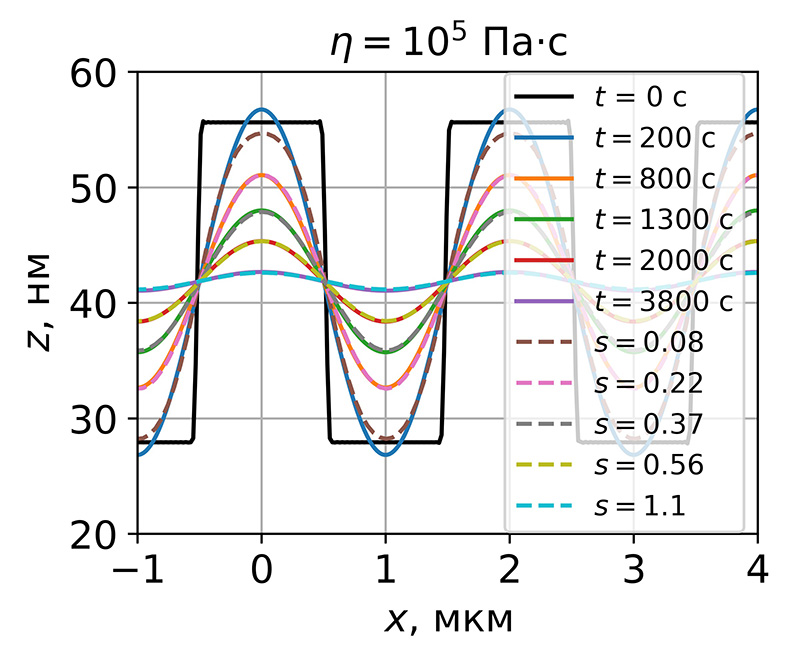
\includegraphics[width=0.91\linewidth]{reflow/grating_eta_100000_14_CORR_200} \\
		\vspace{-28.5ex} \\ \text{\hspace{0em} a}) \\ \vspace{28.5ex}
	\end{minipage}
	\begin{minipage}{0.5\textwidth}
		\hspace{-1em} 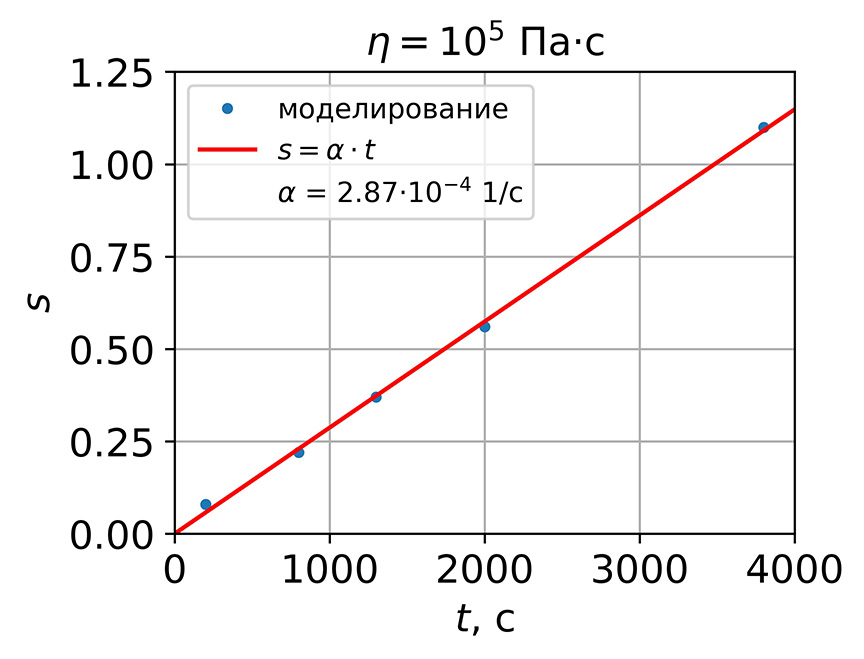
\includegraphics[width=\linewidth]{reflow/alpha_100000_14_up_200} \\
		\vspace{-28.5ex} \\ \text{\hspace{-0.8em} б}) \\ \vspace{28.5ex}
	\end{minipage}
	\vspace{-3.5em}
	\caption{Моделирование растекания прямоугольной решетки с периодом 2 мкм и глубиной 28 нм при значении вязкости материала решетки, равном 10$^\text{5}$~Па$\cdot$с: а) профили решетки, полученные для различных значений времени растекания при моделировании аналитическим (сплошная линия)~\cite{Leveder_2011} и численным (пунктирная линия)~\cite{Brakke_SE} методами; б) зависимость переменной $s$ от времени растекания $t$.}
	\label{fig:reflow_1}
\end{figure}

Вычисление коэффициента $\alpha$ для каждого значения вязкости позволило получить зависимость $\alpha(\eta)$, которая в логарифмических координатах оказалась практически линейной (рисунок~\ref{fig:eta_alpha}). Аппроксимация зависимости $\alpha(\eta)$ функцией вида
\begin{equation}
	\alpha = C / \eta^\beta
\end{equation}
изображена на рисунке~\ref{fig:eta_alpha}, при этом значения параметров $C$ и $\beta$ составили 26.14 и 0.99 соответственно (для значений вязкости в Па$\cdot$с).

\begin{figure}[h]
	\begin{center}
		\includegraphics[width=0.6\textwidth]{reflow/С_gamma_12_SI_200}
	\end{center}
	\vspace{-1.2em}
	\caption{Рассчитанная зависимость коэффициента $\alpha$ от вязкости материала решетки.}
	\label{fig:eta_alpha}
\end{figure}

%Данная зависимость была использована для определения значений подвижности вершин поверхности решетки для различных значений вязкости материала решетки.
При численном моделировании растекания образца программа ``Surface~Evolver'' позволяет отслеживать значение параметра $s$, и логично потребовать, чтобы это значение непосредственно равнялось времени растекания $t$.
Согласно уравнениям~\ref{eq:SE_v} и \ref{eq:SE_v} в этом случае подвижность вершин поверхности решетки $\mu$ может быть выражена следующим образом:
\begin{equation}
	\mu = t / s \equiv \alpha.
\end{equation}
Следовательно, полученная выше зависимость $\alpha(\eta)$ является искомой зависимостью подвижности вершин поверхности резиста от его вязкости, при которой значение переменной $s$ будет равняться времени растекания:
\begin{equation}
	\mu(\eta) \approx \frac{26.14}{\eta}.
\end{equation}
Найденная зависимость позволяет промоделировать растекание сплошной структуры в слое ПММА с неоднородным (в плоскости $XY$) распределением вязкости: сначала на основе распределения вязкости рассчитывается распределение подвижности вершин поверхности структуры, затем в программе ``Surface Evolver'' задается поверхность с определенными значениями подвижности вершин и производится моделирование эволюции поверхности в заданном промежутке значений переменной $s$.

Однако, слой ПММА в процессе СЭЛТР не только имеет неоднородное распределение вязкости, но и является неоднородным в целом.
Как уже было отмечено, в процессе термической деполимеризации в слое ПММА образуется большое количество свободного мономера, который быстро покидает область травления.
Это приводит к появлению микрополостей, объем которых $V_\mathrm{cav}$ может быть вычислен по формуле
\begin{equation}
	V_\mathrm{cav} = N_\mathrm{sci} \cdot 1/\gamma \cdot V_\mathrm{mon},
\end{equation}
где $N_\text{sci}$ -- число разрывов молекул ПММА, $1/\gamma$ -- средняя длина кинетической цепи при деполимеризации, $V_\mathrm{mon}$ -- объем, приходящийся в среднем на один мономер ($\approx$~0.14 нм$\ppp$).
Процессы растекания в методе СЭЛТР протекают за счет действия сил поверхностного натяжения на границах микрополостей в слое \linebreak ПММА, и для возможности применения разработанного подхода для моделирования такого растекания использовалось следующее приближение.
Слой ПММА разделялся в плоскости $XY$ на участки размерами 100$\times$100 нм$\pp$, и для каждого участка на основе промоделированного распределения разрывов молекул \linebreak ПММА и средней длины кинетической цепи при деполимеризации рассчитывались положения и объемы микрополостей (рисунок~\ref{fig:reflow_surface}а).
Далее точки поверхности слоя ПММА, соответствующие середине каждого участка по оси $X$, сдвигались вниз таким образом, чтобы объем призмы, образующейся под поверхностью слоя, был равен суммарному объему микрополостей на этом участке (рисунок~\ref{fig:reflow_surface}б).
Полученная пилообразная структура задавалась в программе ``Surface Evolver'' со значениями подвижности вершин, рассчитанными из распределения вязкости ПММА, усредненному по оси $Z$.
После этого растекание данной структуры моделировалось в течение нужного промежутка времени.

\begin{figure}[h]
	\begin{minipage}{0.48\textwidth}
		\includegraphics[width=0.9\linewidth]{reflow/reflow_model_a_CIRCLES_4} \\
		\vspace{-28.5ex} \\ \text{\hspace{0em} a}) \\ \vspace{28.5ex}
	\end{minipage}
	\begin{minipage}{0.48\textwidth}
		\includegraphics[width=0.9\linewidth]{reflow/reflow_model_b} \\
		\vspace{-28.5ex} \\ \text{\hspace{-0.1em} б}) \\ \vspace{28.5ex}
	\end{minipage}
	\vspace{-3.5em}
	\caption{Иллюстрация подхода к моделированию растекания слоя ПММА со внутренними микрополостями.}
	\label{fig:reflow_surface}
\end{figure}
